\documentclass{standalone}

%----------------------------------------------------------------------------------------------%
%                                 Packages and basic declarations
%----------------------------------------------------------------------------------------------%

\usepackage[utf8]{inputenc}
\usepackage{pgfplots}
\usepackage{tikz}


%----------------------------------------------------------------------------------------------%
%----------------------------------------------------------------------------------------------%
%                                            DOCUMENT STARTS
%----------------------------------------------------------------------------------------------%
%----------------------------------------------------------------------------------------------%

\begin{document}


%Tikz picture starts%

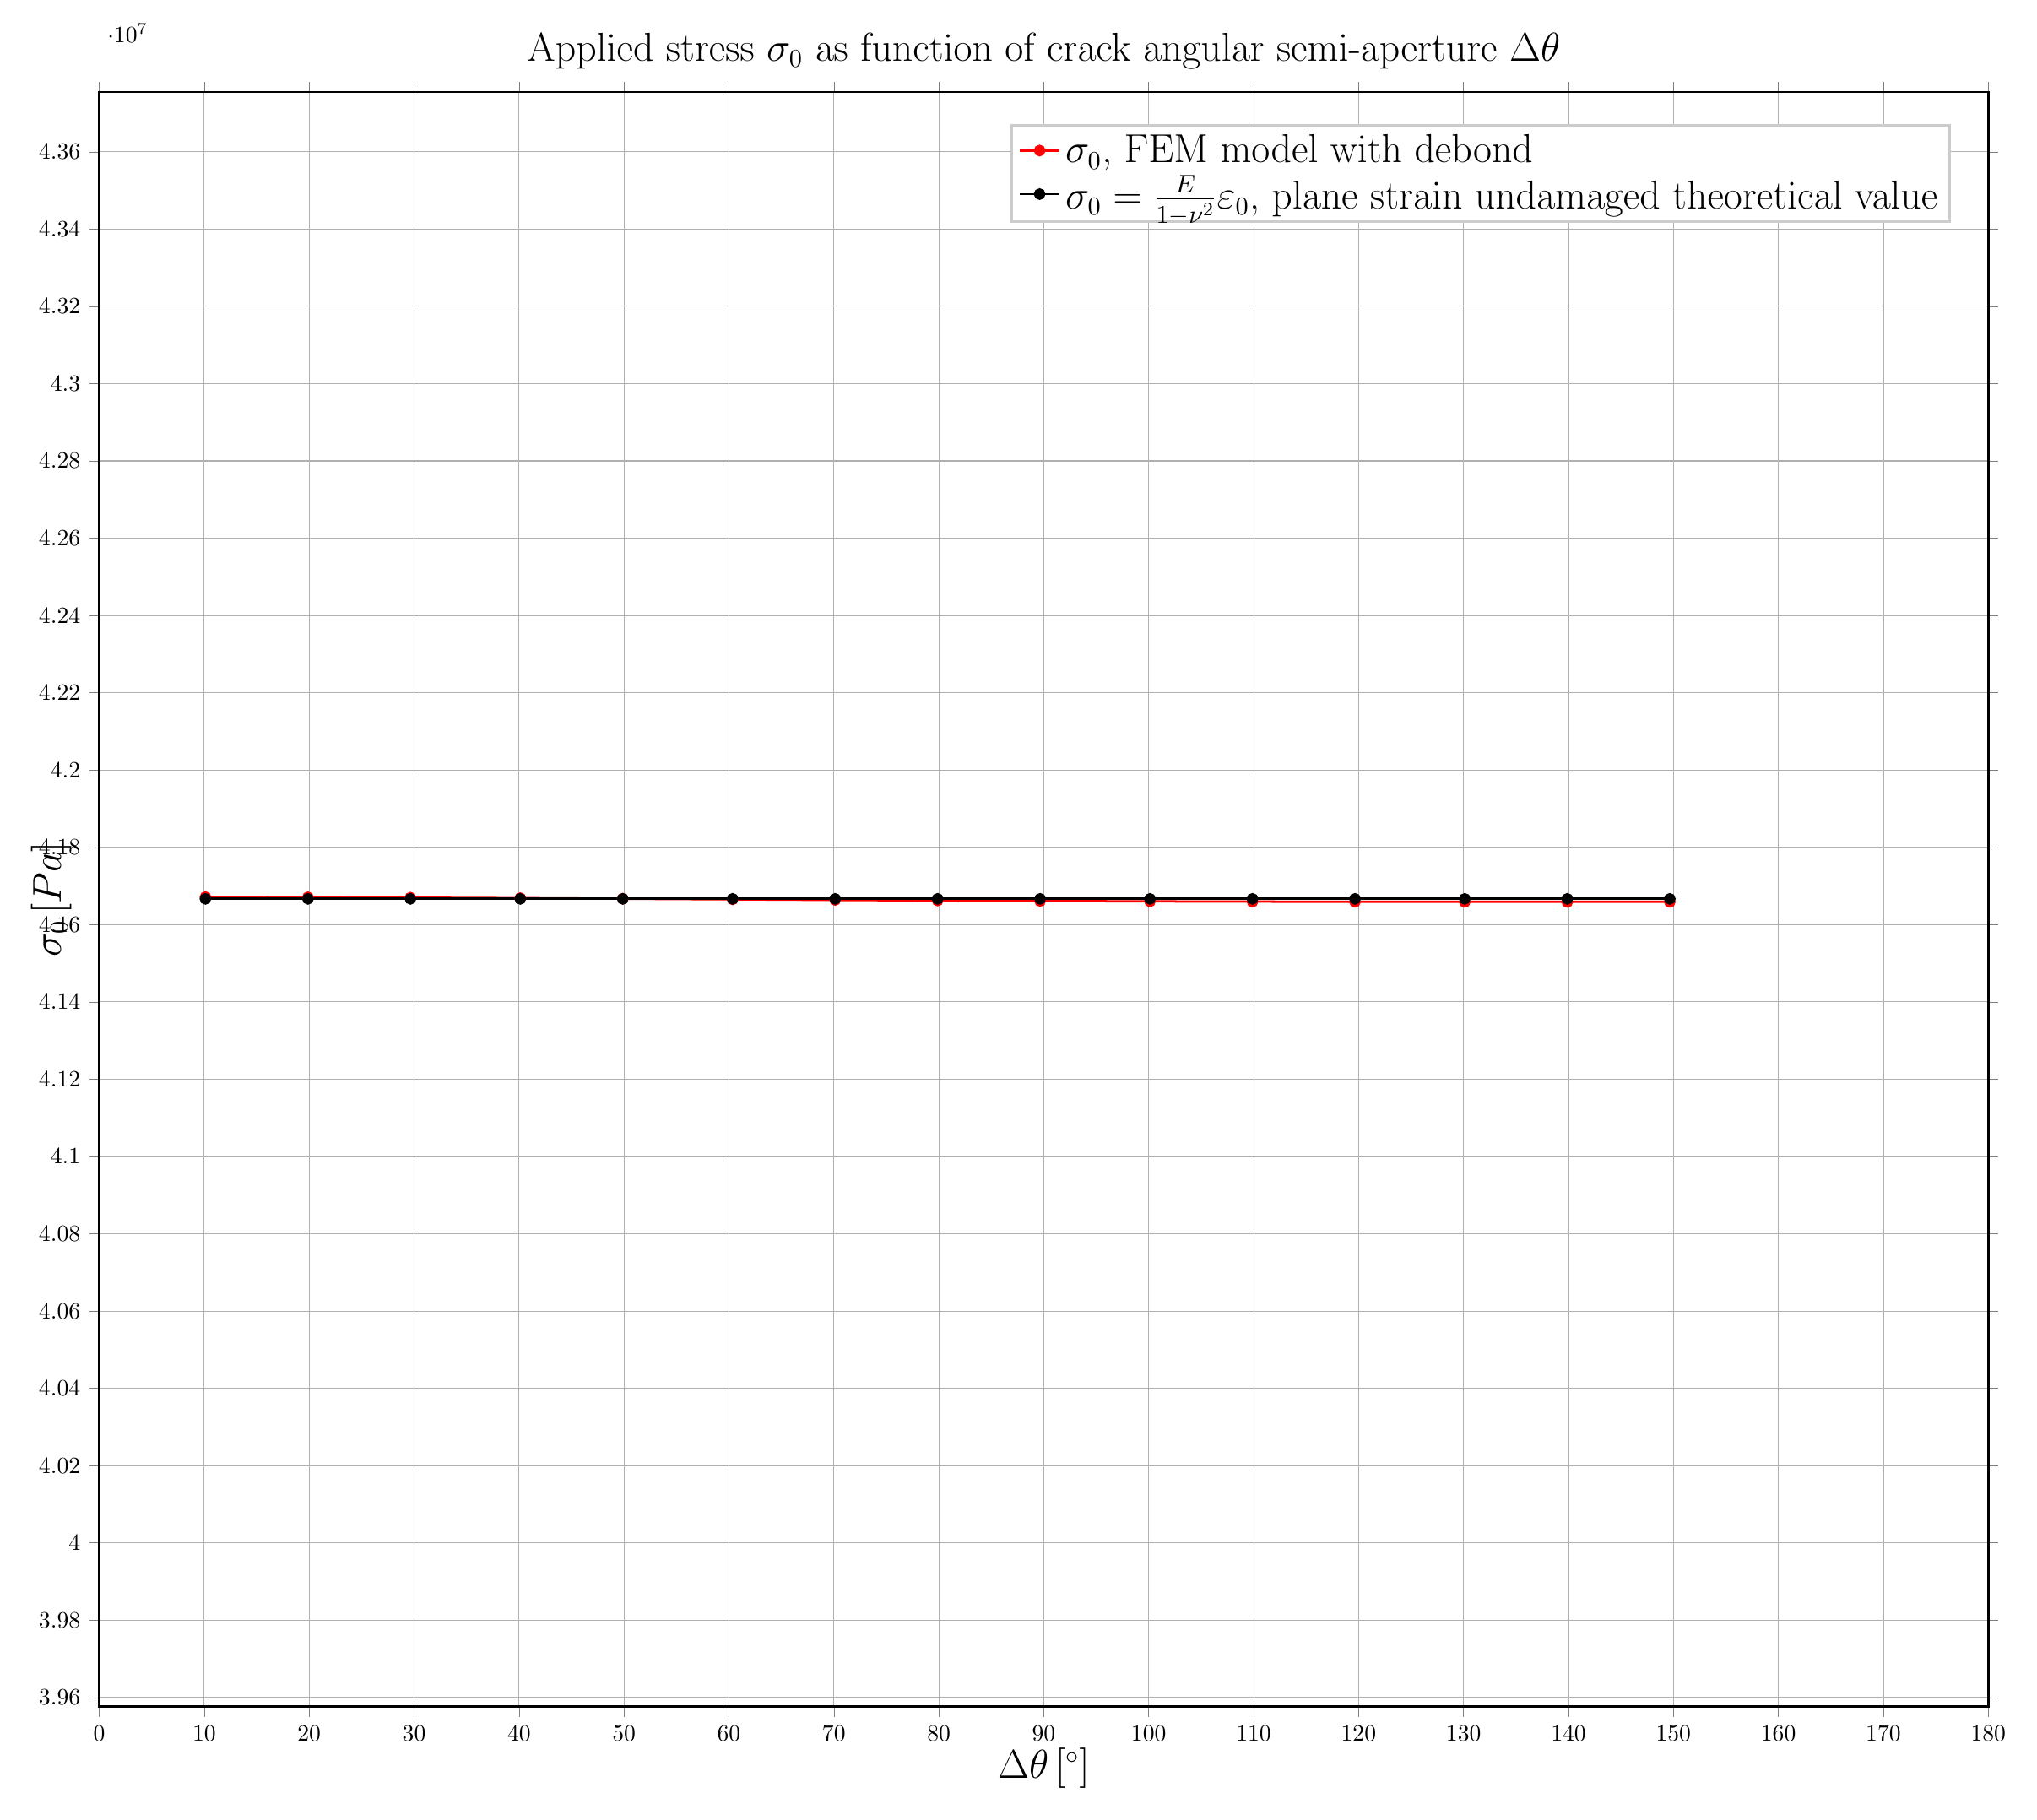
\begin{tikzpicture}

%Tikz axis starts%

\begin{axis}[width=30cm,
title={Applied stress $\sigma_{0}$ as function of crack angular semi-aperture  $\Delta\theta$},
title style={font=\fontsize{16}{8}\selectfont},
xlabel style={at={(axis description cs:0.5,-0.02)},anchor=north,font=\fontsize{16}{8}\selectfont},
ylabel style={at={(axis description cs:-0.01,.5)},anchor=south,font=\fontsize{16}{8}\selectfont},
xlabel={$\Delta\theta\left[^{\circ}\right]$},ylabel={$\sigma_{0}\left[Pa\right]$},
xmin=0.0,
xmax=180.0,
ymin=39576021.1761,
ymax=43754823.6135,
tick align=outside,
tick label style={font=\normalsize},
xtick={0.0,10.0,20.0,30.0,40.0,50.0,60.0,70.0,80.0,90.0,100.0,110.0,120.0,130.0,140.0,150.0,160.0,170.0,180.0},
xmajorgrids,
x grid style={lightgray!92.026143790849673!black},
ymajorgrids,
y grid style={lightgray!92.026143790849673!black},
line width=0.35mm,
legend style={draw=white!80.0!black,font=\fontsize{16}{12}\selectfont},
legend entries={{$\sigma_{0}$, FEM model with debond},{$\sigma_{0}=\frac{E}{1-\nu^{2}}\varepsilon_{0}$, plane strain undamaged theoretical value}},
legend cell align={left}
]

\addplot[red,smooth,mark=*]
table{
10.1165133448 41671260.5843
19.8836864193 41670669.2182
29.6513572437 41669738.9603
40.1161769391 41668439.8651
49.8838221503 41667029.6742
60.3486418456 41665410.0271
70.1163109626 41663890.4425
79.8834883059 41662455.5001
89.651164253 41661171.3703
100.116516703 41660186.7382
109.883687216 41659550.4614
119.651363163 41659191.0289
130.116182859 41659026.6448
139.883817825 41658986.5464
149.651466451 41658983.1132
};

\addplot[black,smooth,mark=*]
table{
10.1165133448 41666666.6667
19.8836864193 41666666.6667
29.6513572437 41666666.6667
40.1161769391 41666666.6667
49.8838221503 41666666.6667
60.3486418456 41666666.6667
70.1163109626 41666666.6667
79.8834883059 41666666.6667
89.651164253 41666666.6667
100.116516703 41666666.6667
109.883687216 41666666.6667
119.651363163 41666666.6667
130.116182859 41666666.6667
139.883817825 41666666.6667
149.651466451 41666666.6667
};

\end{axis}
%Tikz axis ends%


\end{tikzpicture}
%Tikz picture ends%


\end{document}

%----------------------------------------------------------------------------------------------%
%----------------------------------------------------------------------------------------------%
%                                            DOCUMENT ENDS
%----------------------------------------------------------------------------------------------%
%----------------------------------------------------------------------------------------------%

